 \documentclass[12pt,a4paper]{report}
\usepackage[english, polish]{babel}
\usepackage{polski}
\frenchspacing
\usepackage{tabularx}
\usepackage{indentfirst}
\usepackage{xltxtra}
\usepackage{titlesec}
\usepackage{listings}
\usepackage{subcaption}
\usepackage{color}
\definecolor{bluekeywords}{rgb}{0.13,0.13,1}
\definecolor{greencomments}{rgb}{0,0.5,0}
\definecolor{redstrings}{rgb}{0.9,0,0}
\usepackage[margin=25mm,lmargin=30mm,rmargin=20mm]{geometry}
\usepackage{scrpage2}
\usepackage{nameref}
\usepackage[pdfauthor={Marceli Grabowski}, pdftitle={Wieloplatformowa aplikacja mobilna do zakupu biletów kinowych w technologii Xamarin}]{hyperref}
\usepackage[nottoc,notlot,notlof]{tocbibind}
\usepackage{todonotes}
\usepackage{graphicx}
\usepackage{caption}
\usepackage{subcaption}
\usepackage[sorting=none,backend=biber,defernumbers]{biblatex}
\usepackage{float}
\usepackage{pdfpages}
\usepackage[strings]{underscore}
\usepackage{scrhack}
\usepackage{tocbasic}
\addbibresource{bib/bib.bib}
\addbibresource{bib/net.bib}
\setuptoc{lol}{leveldown}
\graphicspath{ {img/} }
\newcommand\todoin[2][]{\todo[inline, caption={2do}, #1]{
\begin{minipage}{\textwidth-4pt}#2\end{minipage}}}
\linespread{1}
\titleformat*{\section}{\fontsize{14pt}{2}\bfseries}
\titleformat*{\subsection}{\fontsize{13pt}{2}\bfseries}
\titleformat*{\subsubsection}{\fontsize{13pt}{2}\bfseries}

\lstset{language=[Sharp]C,
  showspaces=false,
  showtabs=false,
  breaklines=true,
  showstringspaces=false,
  breakatwhitespace=true,
  escapeinside={(*@}{@*)},
  commentstyle=\color{greencomments},
  keywordstyle=\color{bluekeywords},
  stringstyle=\color{redstrings},
  basicstyle=\ttfamily
}

\ifoot[]{}
\cfoot[]{}
\ofoot[\pagemark]{\pagemark}

\pagestyle{scrplain}

\makeatletter
\renewcommand\listoftables{%
    \@mkboth{\MakeUppercase\listtablename}%
        {\MakeUppercase\listtablename}%
    \@starttoc{lot}%
}
\renewcommand\listoffigures{%
    \@mkboth{\MakeUppercase\listfigurename}%
        {\MakeUppercase\listfigurename}%
    \@starttoc{lof}%
}
\renewcommand\lstlistlistingname{Spis listingów}

\makeatother
\renewenvironment{abstract}{
 \vspace*{3cm}
 \begin{center}%
    \bfseries\abstractname
  \end{center}}%
  {\vfill}

\author{Marceli Grabowski}
\title{Wieloplatformowa aplikacja mobilna do zakupu biletów kinowych w technologii Xamarin}

\begin{document}
\linespread{1.3}
\selectfont

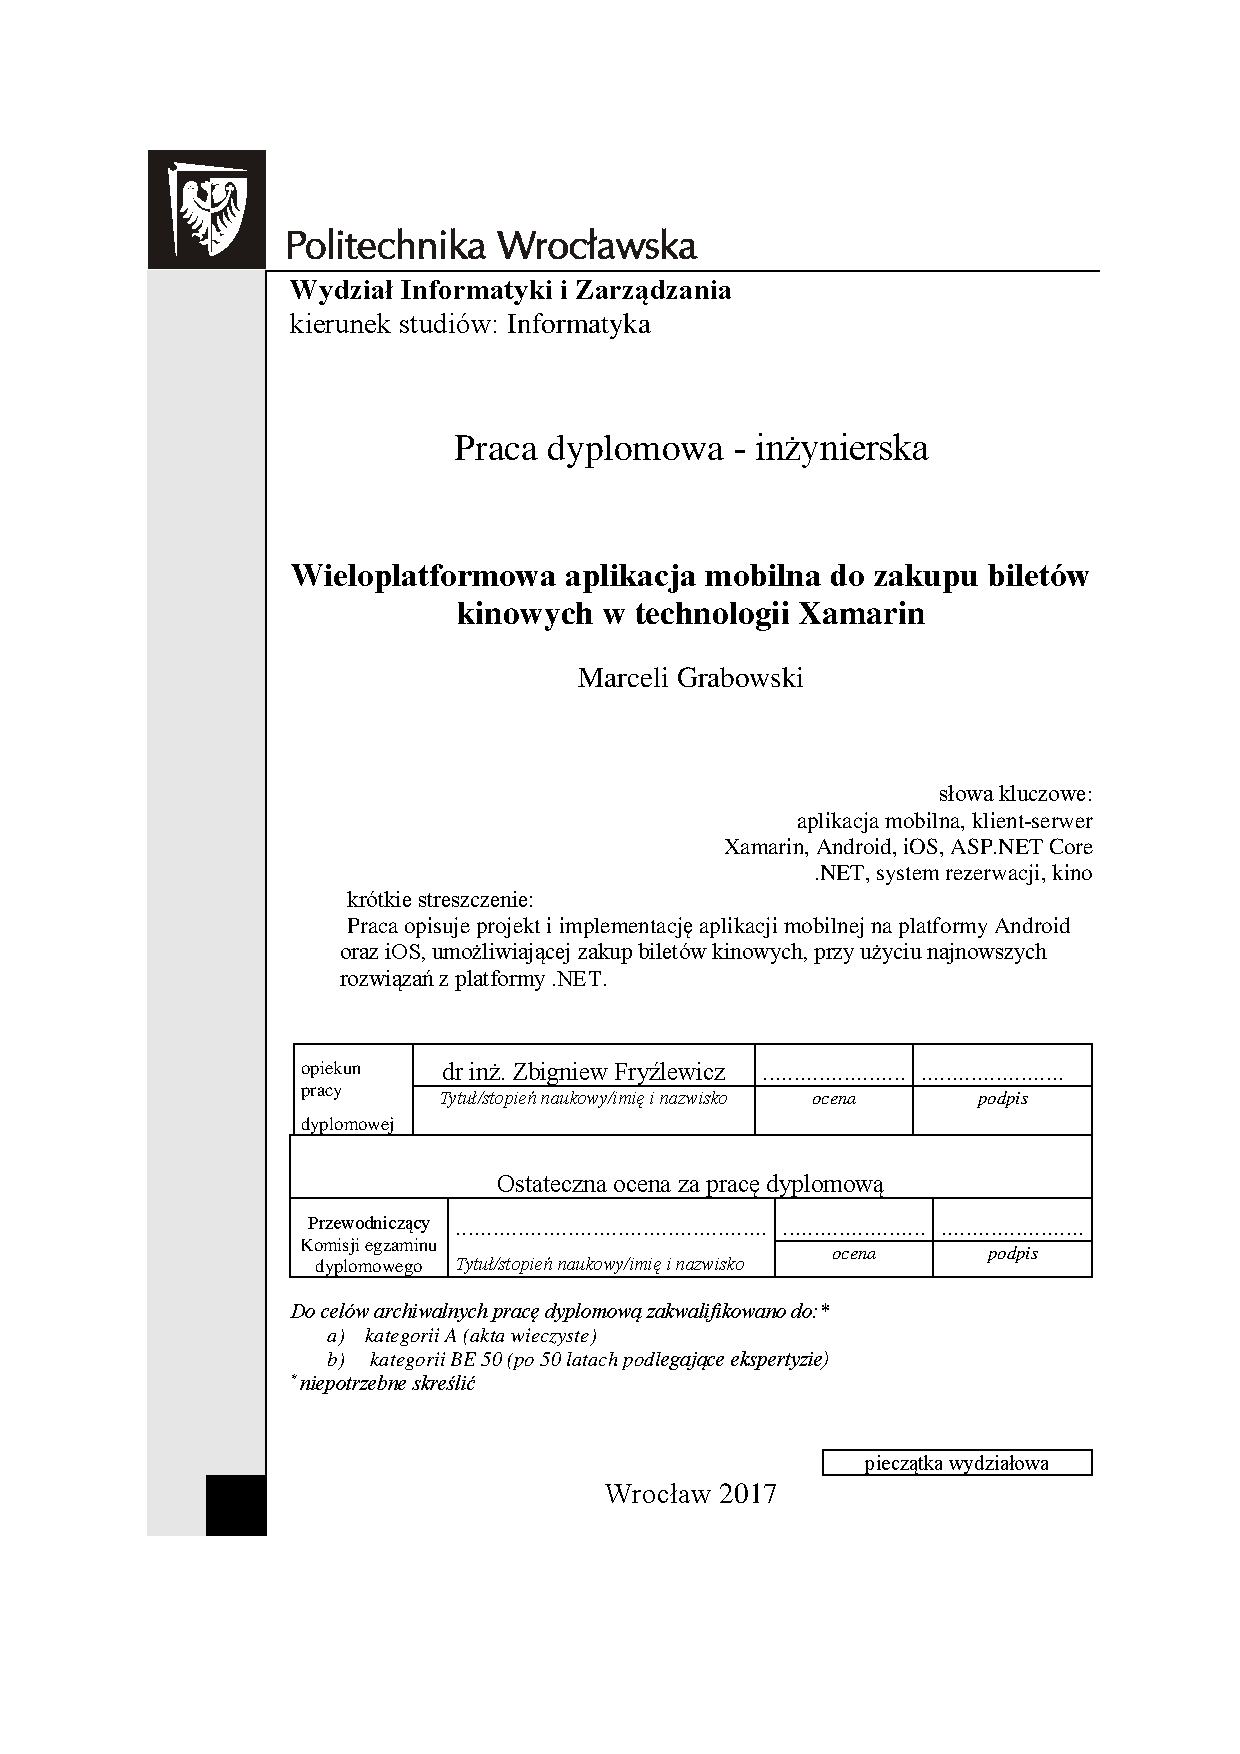
\includepdf[pages={1}]{titlepage.pdf}
\tableofcontents{}

\clearpage
\addcontentsline{toc}{chapter}{Streszczenie}
\abstract{Streszczenie}
\selectlanguage{english}
\abstract{Abstract}
\selectlanguage{polish}
\clearpage

\begin{flushright}
\vspace*{\fill}
\textit{Tu walnij sobie dedykację}
\end{flushright}


\pagebreak

\chapter*{Wstęp}
\chapter{Wprowadzenie do problematyki}
\chapter{Technologie i narzędzia wykorzystywane w pracy}
\section{Xamarin.Android}
\section{Xamarin.iOS}
\section{ASP.NET Core}
\section{Entity Framework Core}
\section{Dapper}
\section{MVVMCross}
\section{AutoFac}
\section{Team Foundation Server}
\section{HockeyApp}
\section{Microsoft Azure}
\chapter{Założenia projektowe}
\section{Przedmiot pracy}
Przedmiotem pracy jest utworzenie aplikacji mobilnej na platformy Android oraz iOS, umożliwiajacej rezerwację i zakup biletów kinowych w ramach sieci kin, wraz z towarzyszącą aplikacją serwerową. Aplikacja kliencka będzie utworzona w oparciu o platformę Xamarin, natomiast aplikacja serwerowa w oparciu o framework ASP.NET Core
\section{Wymagania funkcjonalne}
Oprogramowanie powinno spełniać następujące wymagania funkcjonalne:
\begin{enumerate}
\item Item
\end{enumerate}
\section{Wymagania niefunkcjonalne}
\section{Opis podstawowej architektury systemu}
\chapter{Projekt aplikacji}
\section{Przypadki użycia}
\section{Interfejs}
\section{Diagram klas}
\addtocontents{toc}{\protect\newpage}
\chapter{Implementacja}
\section{DevOps}
\section{Autoryzacja użytkowników aplikacji}
\section{Synchronizacja danych offline-online}
\section{Bezpieczeństwo aplikacji}
\section{Implementacja wzorca CQRS}
\section{Testy interfejsu aplikacji}
\chapter{Podsumowanie}
\chapter*{Bibliografia}
\addcontentsline{toc}{chapter}{Bibliografia}
\chapter*{Załączniki}
\addcontentsline{toc}{chapter}{Załączniki}
\section*{Spis tabel}
\addcontentsline{toc}{section}{Spis tabel}
\section*{Spis rysunków}
\addcontentsline{toc}{section}{Spis rysunków}
\section*{Spis listingów}
\addcontentsline{toc}{section}{Spis listingów}
\section*{Instrukcja kompilacji i testowego uruchomienia aplikacji}
\addcontentsline{toc}{section}{Instrukcja kompilacji i testowego uruchomienia aplikacji}


\end{document}